\documentclass[a4paper,14pt]{extarticle} 
\usepackage[a4paper,top=1.5cm, bottom=1.5cm, left=2cm, right=1cm]{geometry}
%\usepackage[T2A]{fontenc}
%\usepackage[english, russian]{babel}
\usepackage{graphicx}
\graphicspath{{./pics/}}
\DeclareGraphicsExtensions{.pdf,.png,.jpg}

\usepackage{fontspec}
\setmainfont{Times New Roman}
\setsansfont{FreeSans}
\setmonofont{FreeMono}
\renewcommand{\baselinestretch}{1.5}
\usepackage{polyglossia}
\setdefaultlanguage{russian}
\setotherlanguages{english,russian}
\usepackage{setspace}
\usepackage[many]{tcolorbox}
\usepackage{pdfpages}

\usepackage{listings}
\usepackage{xcolor}

\definecolor{codegreen}{rgb}{0,0.6,0}
\definecolor{codegray}{rgb}{0.5,0.5,0.5}
\definecolor{codepurple}{rgb}{0.58,0,0.82}
\definecolor{backcolour}{rgb}{0.95,0.95,0.92}

\lstdefinestyle{mystyle}{
    backgroundcolor=\color{lightgray},
    keywordstyle=\color{magenta},
    frame=single,
    numbers=left,
    numberstyle=\small\color{gray},
    frameround=tttt,
    showspaces=false,
    showstringspaces=false,
    basicstyle=\ttfamily\scriptsize
}

\lstset{style=mystyle}

\begin{document}

    \begin{center}
        \thispagestyle{empty}
        \begin{singlespace}
        ФЕДЕРАЛЬНОЕ АГЕНТСТВО СВЯЗИ

        ФЕДЕРАЛЬНОЕ ГОСУДАРСТВЕННОЕ БЮДЖЕТНОЕ ОБРАЗОВАТЕЛЬНОЕ

        УЧРЕЖДЕНИЕ ВЫСШЕГО ОБРАЗОВАНИЯ

        «САНКТ-ПЕТЕРБУРГСКИЙ ГОСУДАРСТВЕННЫЙ УНИВЕРСИТЕТ ТЕЛЕКОММУНИКАЦИЙ ИМ. ПРОФ. М.А. БОНЧ-БРУЕВИЧА»

        (СПбГУТ)
        \end{singlespace}
        \vspace{-1ex}
        \rule{\textwidth}{0.4pt}
        \vspace{-5ex}

        Факультет \underline{Инфокоммуникационных сетей и систем}

        Кафедра \underline{Защищенных систем связи}
        \vspace{10ex}

        \textbf{Лабораторная работа №7}

    \end{center}
    \vspace{4ex}
    \begin{flushright}
    \parbox{8cm}{
    \begin{flushleft}
        Выполнил:

        \underline{Громов А.А., ИКТЗ-83} \hfill \rule[-0.85ex]{0.1\textwidth}{0.6pt}\\
        \vspace{-1ex}
        \footnotesize \textit{ (Ф.И.О., № группы) \hfill (подпись)} \normalsize

        Проверил:

        \underline{Гельфанд А.М.} \hfill \rule[-0.85ex]{0.1\textwidth}{0.6pt}\\
        \vspace{-1ex}
        (\footnotesize \textit{уч. степень, уч. звание, Ф.И.О.) \hfill (подпись)} \normalsize

    \end{flushleft}
    }
    \end{flushright}
    \begin{center}
        \vfill
        Санкт-Петербург

        2020

        \end{center}

    \newpage

    \begin{center}
        \textbf{8.1.4.7 Packet Tracer - Subnetting Scenario 1}
    \end{center}
    \vspace{-4.3ex}
\begin{lstlisting}[caption=R1 show run]
    version 15.1
    no service timestamps log datetime msec
    no service timestamps debug datetime msec
    no service password-encryption
    hostname R1
    !
    ip cef
    no ipv6 cef
    !
    license udi pid CISCO1941/K9 sn FTX1524V069
    spanning-tree mode pvst
    !
    interface GigabitEthernet0/0
    ip address 192.168.100.1 255.255.255.224
    duplex auto
    speed auto
    !
    interface GigabitEthernet0/1
    ip address 192.168.100.33 255.255.255.224
    duplex auto
    speed auto
    !
    interface Serial0/0/0
    ip address 192.168.100.129 255.255.255.224
    clock rate 64000
    !
    interface Serial0/0/1
    no ip address
    clock rate 2000000
    shutdown
    !
    interface Vlan1
    no ip address
    shutdown
    !
    router eigrp 1
    network 192.168.100.0
    !
    ip classless
    !
    ip flow-export version 9
    !
    line con 0
    !
    line aux 0
    !
    line vty 0 4
    login
    end
\end{lstlisting}

\begin{lstlisting}[caption=S3 show run]
    version 12.2
    no service timestamps log datetime msec
    no service timestamps debug datetime msec
    no service password-encryption
    !
    hostname S3
    !
    spanning-tree mode pvst
    spanning-tree extend system-id
    !
    interface FastEthernet0/1
    .
    .
    .
    interface FastEthernet0/24
    !
    interface GigabitEthernet0/1
    !
    interface GigabitEthernet0/2
    !
    interface Vlan1
    ip address 192.168.100.66 255.255.255.224
    !
    ip default-gateway 192.168.100.65
    !
    line con 0
    !
    line vty 0 4
    login
    line vty 5 15
    login
    !
    end
\end{lstlisting}

\newpage

IP config of pc4

\begin{center}
    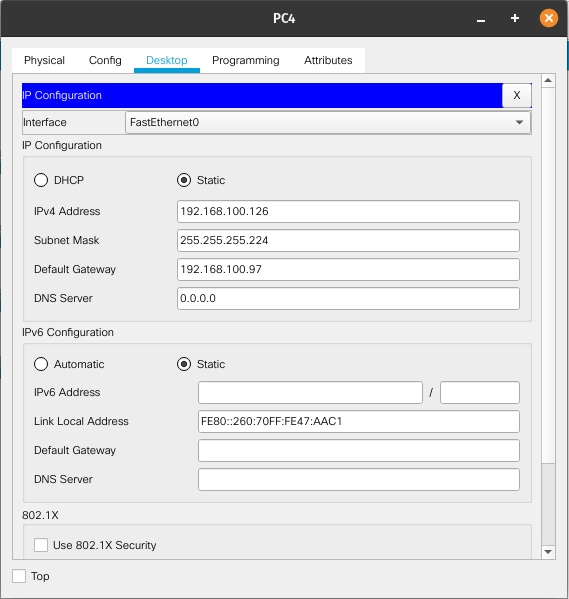
\includegraphics[scale=0.6]{PC4.png}
\end{center}

\newpage
\begin{center}
    \textbf{8.2.1.4 Packet Tracer - Designing and Implementing a VLSM Addressing Scheme}
\end{center}
\vspace{-4.3ex}
\begin{lstlisting}[caption=Branch 1]
    version 15.1
    no service timestamps log datetime msec
    no service timestamps debug datetime msec
    no service password-encryption
    hostname Branch1
    !
    ip cef
    no ipv6 cef
    !
    license udi pid CISCO1941/K9 sn FTX1524V069
    !
    spanning-tree mode pvst
    !
    interface GigabitEthernet0/0
    ip address 10.11.48.97 255.255.255.240
    duplex auto
    speed auto
    !
    interface GigabitEthernet0/1
    ip address 10.11.48.65 255.255.255.224
    duplex auto
    speed auto
    !
    interface Serial0/0/0
    ip address 10.11.48.121 255.255.255.252
    clock rate 64000
    !
    interface Serial0/0/1
    no ip address
    clock rate 2000000
    shutdown
    !
    interface Vlan1
    no ip address
    shutdown
    !
    router eigrp 1
    network 10.11.48.0 0.0.0.255
    !
    ip classless
    !
    ip flow-export version 9
    !
    line con 0
    !
    line aux 0
    !
    line vty 0 4
    login
\end{lstlisting}

\begin{lstlisting}[caption=Branch 2]
    version 15.1
    no service timestamps log datetime msec
    no service timestamps debug datetime msec
    no service password-encryption
    !
    hostname Branch2
    !
    ip cef
    no ipv6 cef
    !
    license udi pid CISCO1941/K9 sn FTX15248AMB
    !
    spanning-tree mode pvst
    !
    interface GigabitEthernet0/0
    ip address 10.11.48.113 255.255.255.248
    duplex auto
    speed auto
    !
    interface GigabitEthernet0/1
    ip address 10.11.48.1 255.255.255.192
    duplex auto
    speed auto
    !
    interface Serial0/0/0
    ip address 10.11.48.122 255.255.255.252
    !
    interface Serial0/0/1
    no ip address
    clock rate 2000000
    shutdown
    !
    interface Vlan1
    no ip address
    shutdown
    !
    router eigrp 1
    network 10.11.48.0 0.0.0.255
    !
    ip classless
    !
    ip flow-export version 9
    !
    line con 0
    !
    line aux 0
    !
    line vty 0 4
    login
    !
    end
\end{lstlisting}
\newpage
\begin{lstlisting}[caption=Room-312]
    version 12.2
    no service timestamps log datetime msec
    no service timestamps debug datetime msec
    no service password-encryption
    !
    hostname Room-312
    !
    spanning-tree mode pvst
    spanning-tree extend system-id
    !
    interface FastEthernet0/1
    .
    .
    .
    interface FastEthernet0/24
    !
    interface GigabitEthernet0/1
    !
    interface GigabitEthernet0/2
    !
    interface Vlan1
    ip address 10.11.48.114 255.255.255.248
    !
    ip default-gateway 10.11.48.113
    !
    line con 0
    !
    line vty 0 4
    login
    line vty 5 15
    login
    !
    end
\end{lstlisting}
\newpage

IP config PC-D
\begin{center}
    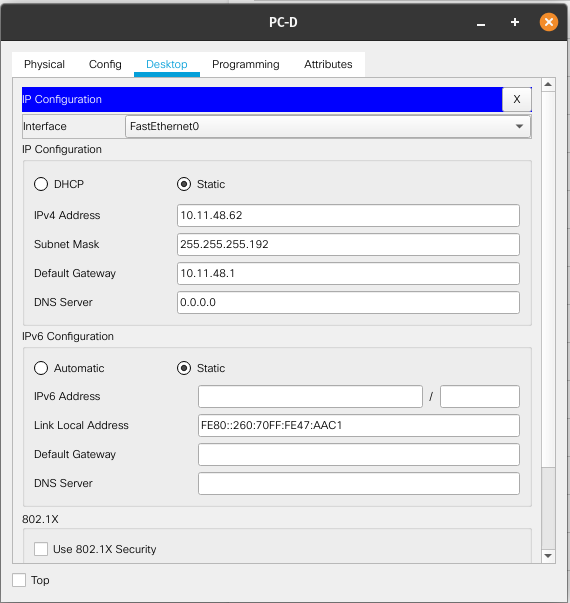
\includegraphics[scale=0.5]{PC-D}
\end{center}

\end{document}